%------------------------------------------------------------------------------------------------
%Listen
%------------------------------------------------------------------------------------------------
\section{Listen}
\subsection{Eigenschaften von Listen}
\begin{itemize}
  \item Unterschied Array $\leftrightarrow$ Liste :
  	\begin{itemize}
	  	\item Array: Anzahl Elemente \textbf{statisch} 
	  	\item Liste: Anzahl Elemente \textbf{dynamisch}
  	\end{itemize}
  \item Listenelement = Knoten oder Node
  \item Listenanfang: Muss immer gegeben sein, da von diesem ausgegangen wird. 
  \item Listenende: Wird durch Nullpointer definiert
\end{itemize}
%------------------------------------------------------------------------------------------------



%------------------------------------------------------------------------------------------------
%Single Linked Lists
%------------------------------------------------------------------------------------------------
\subsection{Einfach verkettete Liste - Single Linked List}
\begin{flushleft}
{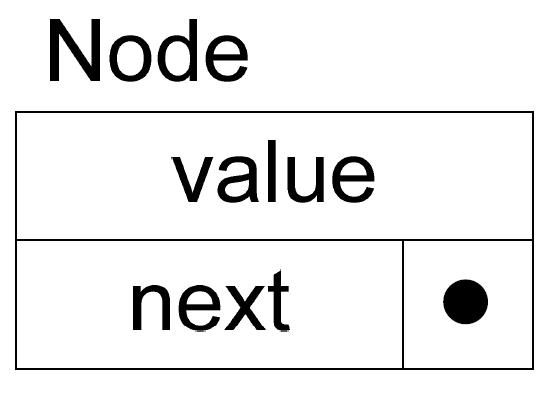
\includegraphics[width=0.1\textwidth]{images/Listen/SLL.png}}
\label{Fig: Single Linked List}
\end{flushleft}
\subsubsection{Definition Node}
\begin{lstlisting}[style=C]
struct Node
{
	Item value; //Gespeicherte Wert, z.Bsp. double
	Node* next; //Pointer auf na"chstes Listenelement
};
\end{lstlisting}

\subsubsection{Definition Listenanfang}
\begin{lstlisting}[style=C]
Node* pHead; //Kopf der Liste
\end{lstlisting}

\subsubsection{Listenelement einf"ugen}
\begin{lstlisting}[style=C]
void SList::insertAt(int pos,double val)
{
	assert(pos >= 0);
	Node* pEl = new Node;
	pEl->value = val;
	if (pos != 0)
	{
		Node* p = nodePtr(pos);
		assert(p != 0);
		pEl->next = p->next;
		p->next = pEl;
	}
	else // insert at head
	{
		pEl->next = pHead;
		pHead = pEl;
	}
	++nr;
}
\end{lstlisting}
\begin{flushleft}
{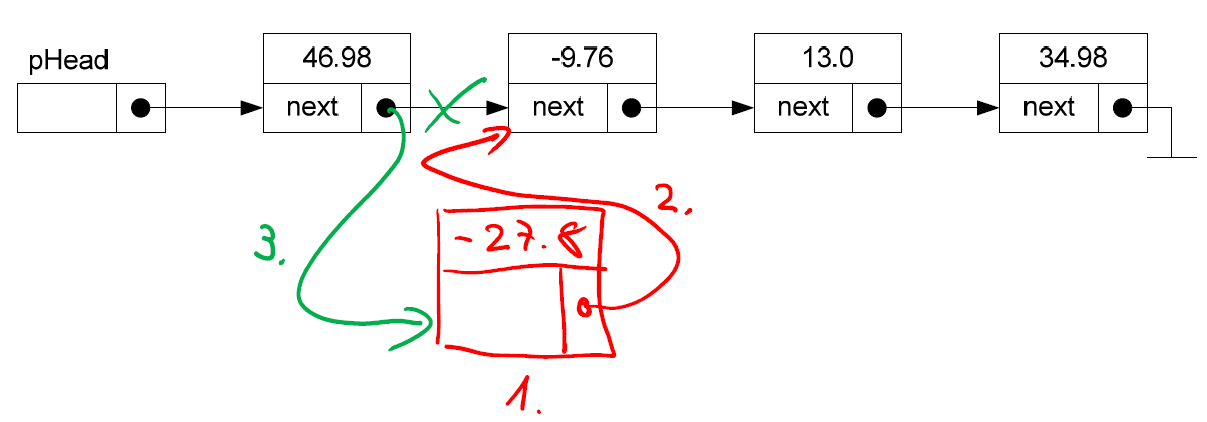
\includegraphics[width=0.5\textwidth]{images/Listen/SLL_Insert.png}}
\label{Fig: Element bei SLL einf"ugen}
\end{flushleft}

\subsubsection{Listenelement l"oschen}
\begin{lstlisting}[style=C]
void SList::deleteAt(int pos)
{
	assert(pos > 0 && pos <= nr);
	Node* p = pHead; // cursor
	Node* pDel = p; // node to be deleted
	if (pos == 1) // first element
		pHead = pHead->next;
	else
	{
		for (int i = 1; i < pos-1; i++)
		{
			p = p->next;
		}
		pDel = p->next;
		p->next = pDel->next;
	}
	delete pDel;
	--nr;
}
\end{lstlisting}
\begin{flushleft}
{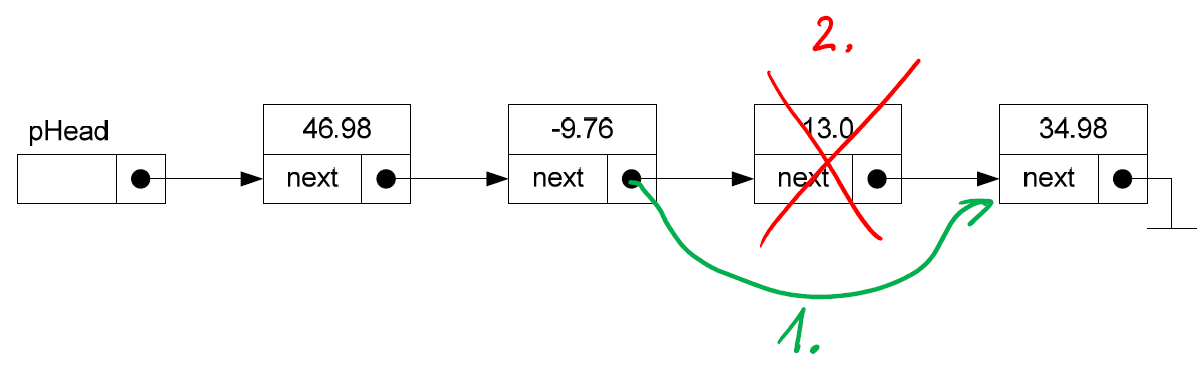
\includegraphics[width=0.5\textwidth]{images/Listen/SLL_Delete.png}}
\label{Fig: Element bei SLL l"oschen}
\end{flushleft}

\subsubsection{Listenelement suchen}
\begin{lstlisting}[style=C]
int SList::search(double val) const
{
	Node* p = pHead; // p points to element at pos 1, if not empty
	for (int i = 1; p; i++)
	{
		if (p->value == val)
		{
			return i;
		}
		p = p->next;
	}
	return 0; // not found
}
\end{lstlisting}
%------------------------------------------------------------------------------------------------



%------------------------------------------------------------------------------------------------
%Double Linked Lists
%------------------------------------------------------------------------------------------------
\subsection{Doppelt verkettete Liste - Double Linked List}
\begin{flushleft}
{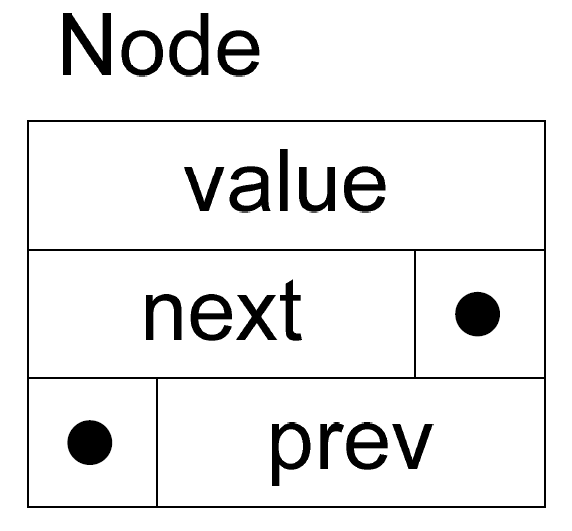
\includegraphics[width=0.1\textwidth]{images/Listen/DLL.png}}
\label{Fig: Double Linked List}
\end{flushleft}
\subsubsection{Definition Node}
\begin{lstlisting}[style=C]
struct Node
{
	Item value; // der gespeicherte Wert, z.B. double
	Node* next; // Pointer auf das naechste Listenelement
	Node* prev; // Pointer auf das vorheriges Listenelement
};
\end{lstlisting}

\subsubsection{Listenelement einf"ugen}
\begin{lstlisting}[style=C]
void DList::insertAt(int pos,double val)
{
	assert(pos >= 0);
	Node* pEl = new Node;
	pEl->value = val;
	if (pos != 0)
	{
		Node* p = nodePtr(pos);
		assert(p != 0);
		pEl->next = p->next;
		pEl->prev = p;
		p->next = pEl;
	}
	else // insert at head
	{
		pEl->next = pHead;
		pEl->prev = 0;
		pHead = pEl;
	}
	if (pEl->next != 0) // not last element in list
	{
		pEl->next->prev = pEl;
	}
	++nr;
}
\end{lstlisting}
\begin{flushleft}
{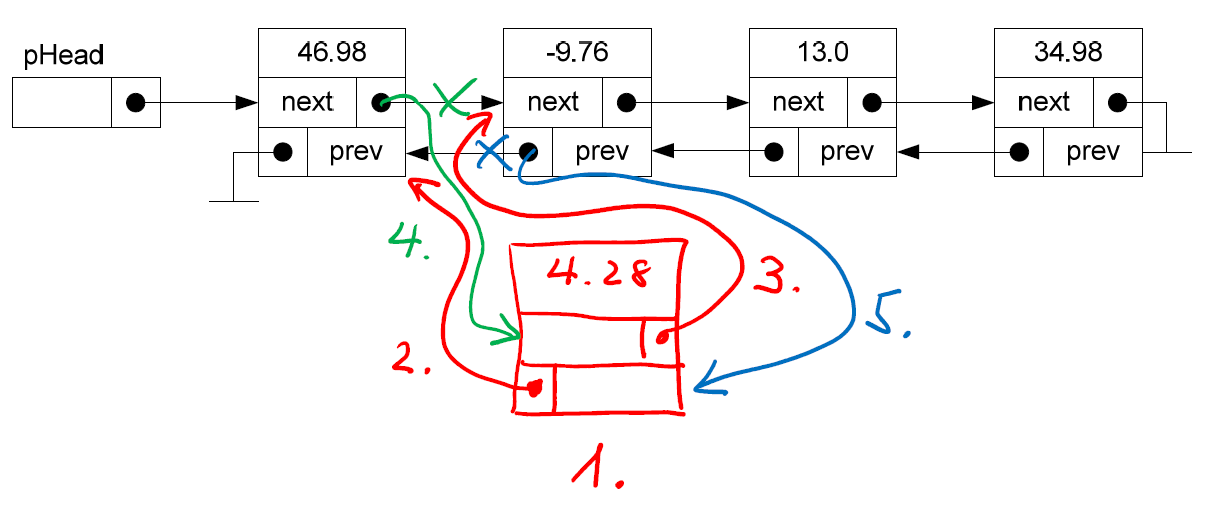
\includegraphics[width=0.5\textwidth]{images/Listen/DLL_Insert.png}}
\label{Fig: Element bei DLL einf"ugen}
\end{flushleft}

\subsubsection{Listenelement l"oschen}
\begin{lstlisting}[style=C]
void DList::deleteAt(int pos)
{
	assert(pos > 0 && pos <= nr);
	Node* pDel = nodePtr(pos); // node to be deleted
	assert (pDel != 0);
	if (pos == 1) // first element
		pHead = pHead->next;
	else
	{
		pDel->prev->next = pDel->next;
	}
	if (pDel->next != 0) // not last element in list
	pDel->next->prev = pDel->prev;
	delete pDel;
	--nr;
}
\end{lstlisting}
\begin{flushleft}
{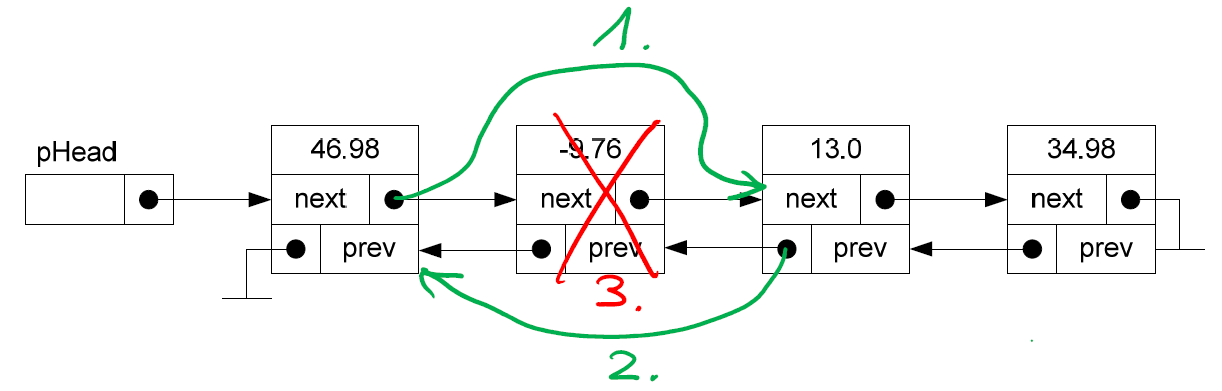
\includegraphics[width=0.5\textwidth]{images/Listen/DLL_Delete.png}}
\label{Fig: Element bei DLL l"oschen}
\end{flushleft}

\subsubsection{Listenelement suchen}
\begin{lstlisting}[style=C]
int DList::search(double val) const
{
	Node* p = pHead; // p points to element at pos 1, if not empty
	for (int i = 1; p; i++)
	{
		if (p->value == val)
		{
			return i;
		}
		p = p->next;
	}
	return 0; // not found
}
\end{lstlisting}
